\documentclass[twocolumn]{article}
\usepackage{graphicx}
\usepackage[a4paper, left=1.5in, right=1.5in]{geometry}

\title{A Deep Dive into OpenVAS: Enhancing Your Network's Security Through Effective Vulnerability Scanning and Risk Mitigation}
\author{Nikola Dinevski, nikola.dinevski@yahoo.com}\\
\date{December 2024}

\begin{document}

\maketitle

\textbf{Abstract - This paper explores the capabilities of OpenVAS (Open Vulnerability Assessment System) as a comprehensive tool for vulnerability scanning and risk mitigation in network security. By implementing OpenVAS in a corporate network environment, this study examines its practical application, highlighting its strengths in identifying security vulnerabilities and providing actionable insights for remediation. The paper talks about the benefits of OpenVAS, including its scalability, open-source nature, and ease of integration with existing security frameworks. However, it also addresses the tool's limitations, such as performance issues in large networks and the need for manual intervention in certain cases. Through real-world implementation and analysis, this paper aims to provide a thorough understanding of OpenVAS as a crucial component in enhancing network defenses and reducing cybersecurity risks.}

\vspace{0.25em}

\textbf{Keywords:} OpenVAS, Vulnerability Scanning, Network Security, Risk Mitigation, Cybersecurity, Vulnerability Assessment, Network Defense, Security Tools

\section{Introduction}
The need for robust vulnerability scanning and network security has never been more pressing, as cyber threats become increasingly sophisticated. Companies are seeking to protect their sensitive data and digital infrastructure. As cyber threats grow increasingly sophisticated, the need for effective vulnerability scanning and risk mitigation tools becomes ever more critical. In this paper, I present the implementation of OpenVAS, an open-source vulnerability scanner, within my company's network, highlighting its utility in identifying security weaknesses and potential entry points for attackers.

OpenVAS is a comprehensive and flexible tool for vulnerability assessment, capable of scanning networks, servers, and applications for security flaws. By scanning my company’s network with OpenVAS, I aimed to evaluate the tool’s effectiveness in detecting vulnerabilities, understanding the scanning process, and identifying any potential weaknesses in the system. This implementation is particularly important as it provides real-world insights into how OpenVAS functions in a live enterprise network, where the complexity of systems and devices can pose challenges.

Through this paper, I will walk through the steps I followed in deploying OpenVAS, analyzing the results of the scans, and discussing the various vulnerabilities that were discovered. The goal is to demonstrate how OpenVAS enhances an organization’s security posture and the lessons learned from applying the tool in a real-world environment.

\section{OpenVAS}

OpenVAS (Open Vulnerability Assessment System) is a free, open-source vulnerability scanner designed for performing comprehensive network vulnerability assessments. It is widely used by security professionals to identify potential vulnerabilities within a network and help organizations improve their cybersecurity posture.

OpenVAS offers various features that make it a powerful tool for vulnerability management:

\begin{itemize}
    \item Free and Open-Source: OpenVAS is freely available and open-source, which allows anyone to use, modify, and contribute to its development. This makes it a highly accessible solution for organizations of all sizes.
    \item Comprehensive Vulnerability Scanning: It provides a wide range of scanning options, including authenticated and unauthenticated scans, and can check for vulnerabilities across various operating systems, devices, and services.
    \item Regular Updates: OpenVAS is regularly updated with new vulnerability tests (VTs) to ensure that it stays up-to-date with the latest known vulnerabilities.
    \item Customizable and Extensible: The platform allows for customization in terms of scan configurations, report formats, and integrates with other security tools via the Greenbone Management Protocol (GMP).
    \item Web Interface: It provides a user-friendly web interface for managing scans, analyzing results, and managing vulnerabilities. The interface is intuitive and allows for easy access to detailed reports.
\end{itemize}

OpenVAS includes a detailed reporting system that categorizes vulnerabilities based on severity and provides actionable recommendations for remediation. It also supports compliance scans and special scans, making it suitable for a variety of use cases, including regulatory compliance.

\subsection{Components and Field of Application}

The OpenVAS framework includes several key components:

\begin{itemize}
    \item Greenbone Enterprise Appliance (GOS): A hardware or virtual appliance that runs Greenbone OS (GOS), which is used for vulnerability scanning and management. 
    \item Greenbone Vulnerability Management (GVM): The core component responsible for managing vulnerability tests, tasks, and reports.
    \item Greenbone Management Protocol (GMP): A protocol used for interacting with OpenVAS remotely and automating vulnerability management tasks.
\end{itemize}

The field of application for OpenVAS is vast. It is applicable in network security, system administration, and compliance audits. It can scan systems such as Linux, Windows, network devices, and web applications to identify vulnerabilities and risks. 

\subsection{Types of Scans Offered by OpenVAS}

OpenVAS supports various types of vulnerability scans, including:

\begin{itemize}
    \item Authenticated Scans: These scans use credentials to access target systems and perform a deeper assessment of system vulnerabilities.
    \item Unauthenticated Scans: These scans do not require credentials and identify vulnerabilities that can be exploited without user authentication.
    \item CVEs and CPE-Based Scans: OpenVAS can check systems for specific Common Vulnerabilities and Exposures (CVEs) and Common Platform Enumeration (CPE) based checks.
    \item Compliance Scans: These scans evaluate the security of systems against established compliance frameworks such as IT-Grundschutz or BSI TR-03116.
    \item Container Scans: OpenVAS can also perform scans on containerized environments to ensure they are secure and free of vulnerabilities.
\end{itemize}

\subsection{Vulnerability Classification and Elimination}

Once vulnerabilities are identified, OpenVAS classifies them based on their severity, typically categorizing them into levels such as low, medium, high, and critical. The system also provides detailed remediation guidance, including patches and configuration changes needed to mitigate the identified vulnerabilities.

Reports generated by OpenVAS can be customized to include specific vulnerabilities, compliance results, or remediation suggestions, making it easier for organizations to prioritize their security efforts.

\subsection{Why OpenVAS?}

OpenVAS is a versatile, scalable solution that provides organizations with the tools to identify, manage, and remediate vulnerabilities effectively. Whether you are conducting routine security assessments or preparing for compliance audits, OpenVAS offers the capabilities necessary to enhance your network security posture.

\section{Implementation}

\subsection{Installation and Setup}

To begin, I started an Ubuntu VM and I set the Network Adapted in Bridged Mode, which basically allowed the VM to get a private IP Address from the local network. This is really important since it allows the VM to ping all devices connected to the said network. OpenVAS was installed (Fig. 1) and configured to meet the specific requirements of my company's network environment. The version of OpenVAS used for the implementation was v22.4, which was selected based on its stability and feature set. The installation process involved setting up the Greenbone Vulnerability Management (GVM) suite, which includes the OpenVAS scanner and Greenbone Security Assistant (GSA) for managing and reviewing scans. I used the official docker-compose.yml from Greenbone to run the containers (Fig. 2). An important thing to note, is that to each container, $$network\_mode: "host"$$ should be added to allow all of the containers be treated as separate machines in the network. The point of this is that they get a private IP Address from the local network, which will allow them to ping all devices inside this network (Fig. 3).

\begin{figure}[h!]
    \centering
    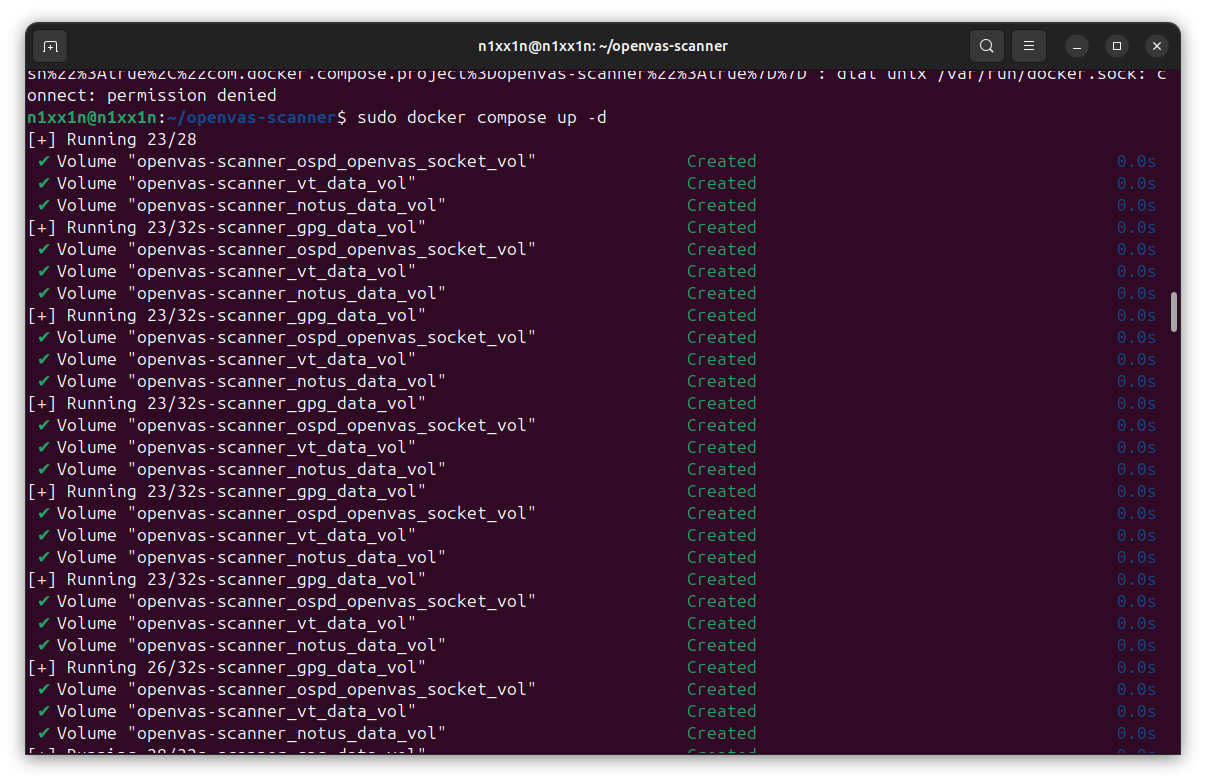
\includegraphics[width=0.5\textwidth]{dockerrun.png}
    \caption{Installation}
\end{figure}

\begin{figure}[h!]
    \centering
    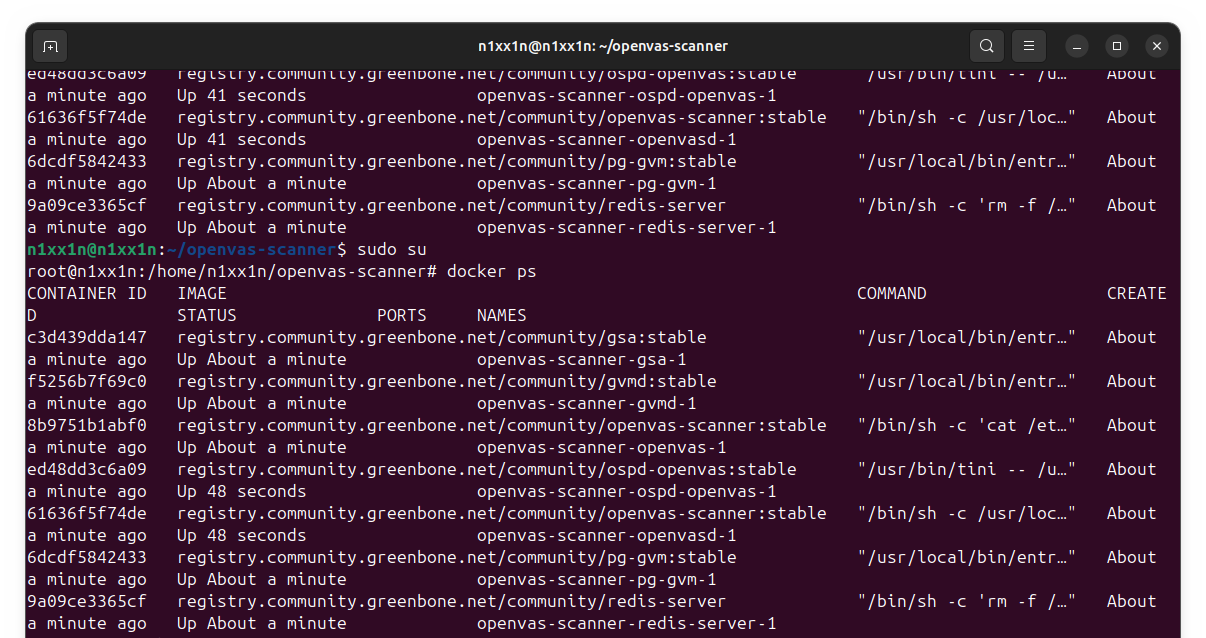
\includegraphics[width=0.5\textwidth]{dockerps.png}
    \caption{Running}
\end{figure}

\begin{figure}[h!]
    \centering
    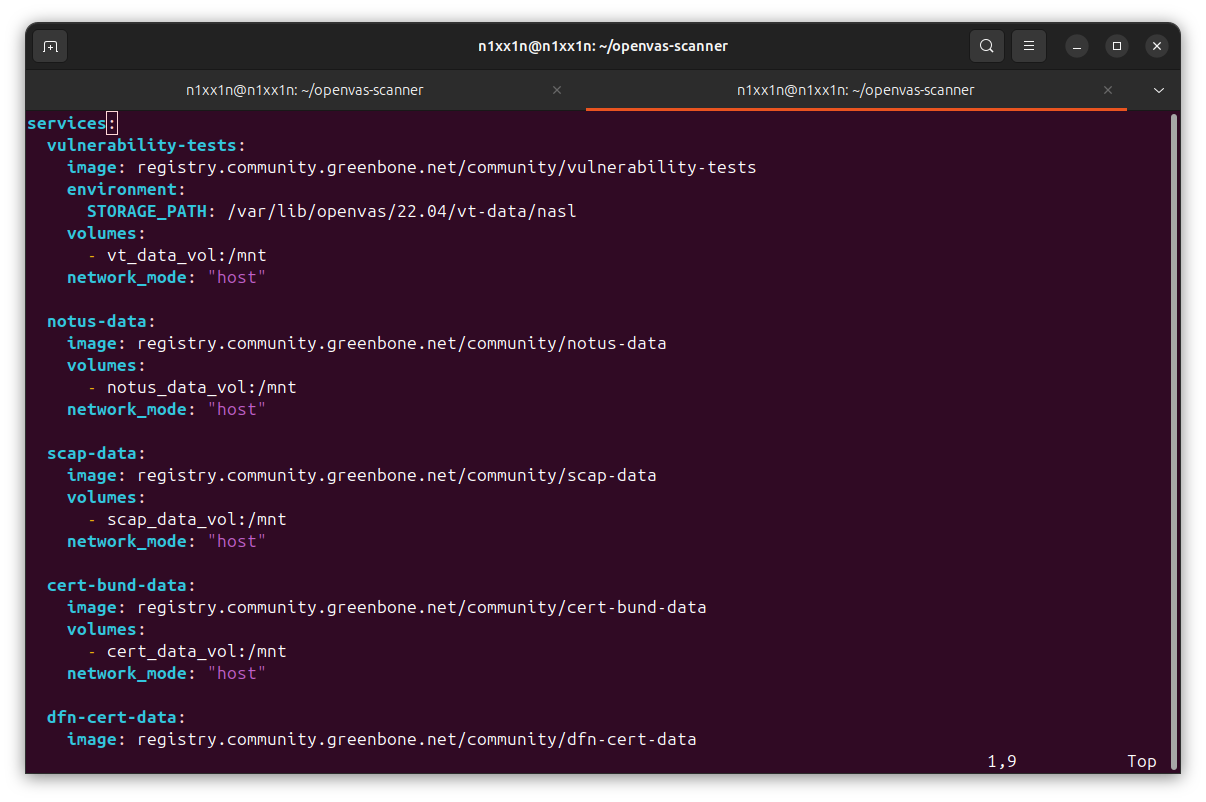
\includegraphics[width=0.5\textwidth]{yaml.png}
    \caption{docker-compose.yml}
\end{figure}

\subsubsection{Dependencies and Configuration:}

OpenVAS requires several dependencies, such as PostgreSQL for the database, Redis for caching, and a variety of security tools to perform the vulnerability scanning.

Now, after the containers were up and running, I could access the interface that OpenVAS provides. And from inside the container I could ping other devices on the private network, ensuring access to all of the devices. After logging in (Fig. 4) and further navigating to the Feed Status Page, we can notice that the CVEs, CPEs, CERTs, Policies, Configs, NVTs updates are in progress (Fig. 5). 

\begin{figure}[h!]
    \centering
    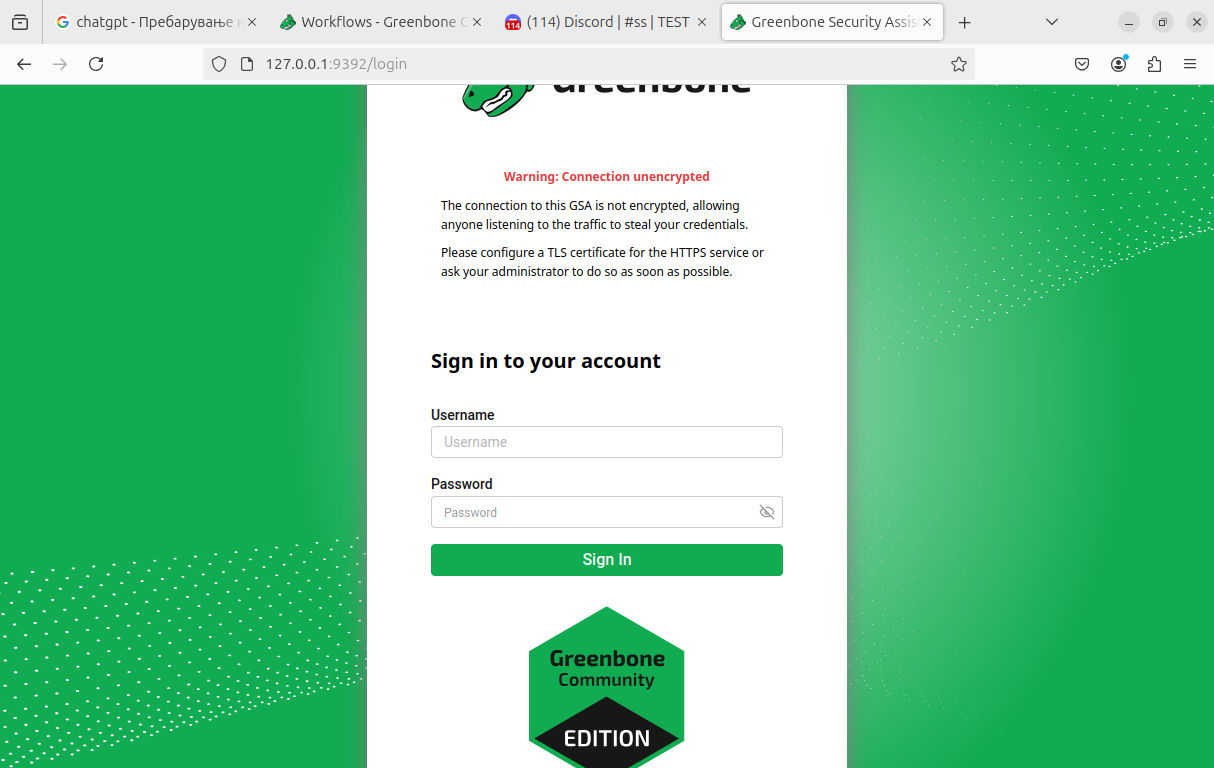
\includegraphics[width=0.5\textwidth]{login.png}
    \caption{Login Page}
\end{figure}

\begin{figure}[h!]
    \centering
    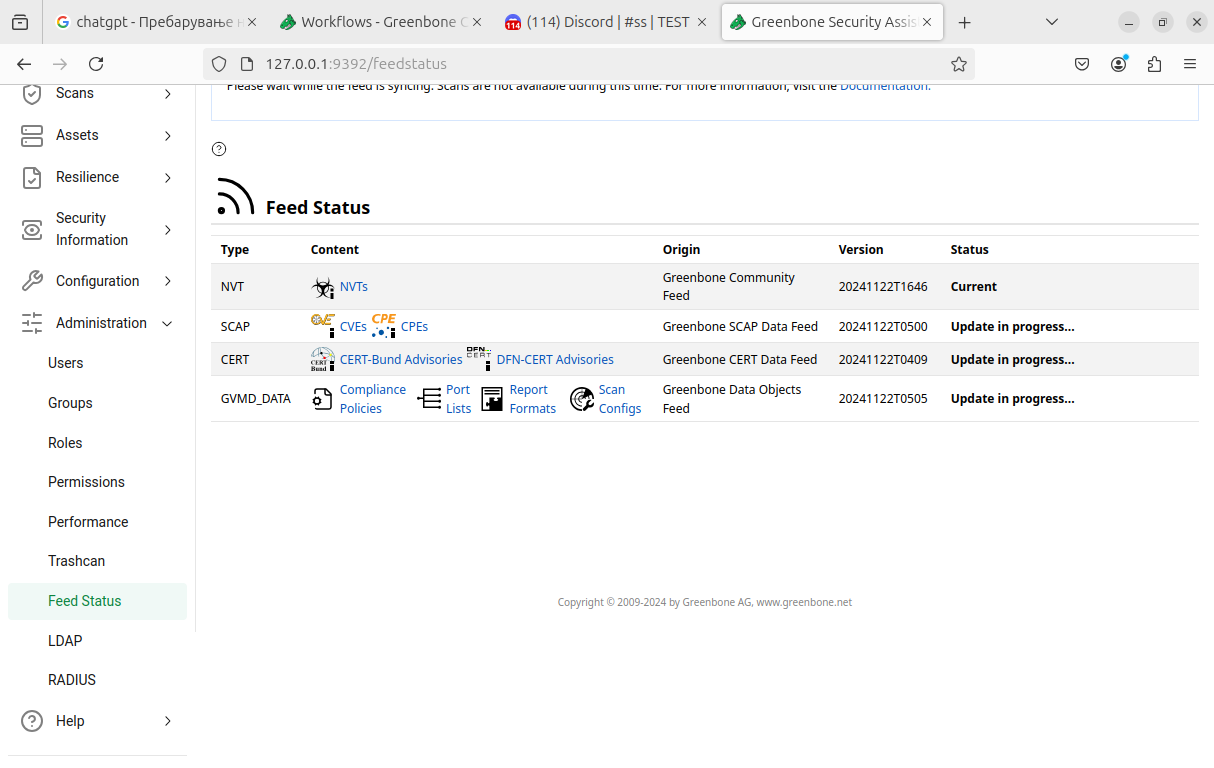
\includegraphics[width=0.5\textwidth]{update.png}
    \caption{Feed Status Page}
\end{figure}

\subsection{Network Environment}

Our company’s network is composed of several types of devices:

\begin{itemize}
    \item \textbf{Servers:} These include web servers, application servers, and file servers, all running a combination of Linux and Windows Server operating systems.
    \item \textbf{Workstations:} Primarily Windows 10/11 and macOS machines used by employees for day-to-day activities.
    \item \textbf{Other devices:} Any other device that is connected to the network ( laptops, mobile devices, printers, etc. )
\end{itemize}

The network is structured across multiple subnets, which with a quick check I found out that excluding the network (192.168.100.0) and broadcast (192.168.101.255) addresses, the usable range is
192.168.100.1 to 192.168.101.254. Which means that for now, to "catch" all devices connected on this network, we should set up the scans for this range.

\subsection{Scanning Configuration}

Given the complexity of the network, I used a mix of scanning techniques to ensure comprehensive coverage and to accurately identify vulnerabilities across various system types.

\subsubsection{Scan Overview:}

\begin{itemize}
    \item \textbf{Full Scans:} These were run periodically across our entire network to provide an overall assessment of vulnerabilities, including both authenticated and unauthenticated scans.
    \item \textbf{Authenticated Scans:} For critical servers and databases, I set up authenticated scans, allowing OpenVAS to access the system as an authenticated user to discover vulnerabilities that are not visible in unauthenticated scans.
    \item \textbf{Custom Scans:} I created tailored scans to focus on specific vulnerabilities, such as SSL/TLS configuration issues or missing patches, particularly in sensitive systems like public-facing web servers.
\end{itemize}

\subsubsection{Initial Configuration:}

A few initial configurations were needed to tailor OpenVAS to our company’s network architecture. These included setting up specific scanning targets (i.e., network segments, servers, and workstations) and enabling features such as authenticated scans to ensure deeper vulnerability detection. Custom scan configurations were also created to optimize the scanning process based on the criticality of systems, ensuring that more sensitive infrastructure was prioritized during scans.

\subsection{Scans}

The process of creating and configuring the scans was a key part of the implementation of OpenVAS in my company's network. The primary goal was to ensure comprehensive coverage of all devices within our network, identifying potential vulnerabilities in critical systems and enabling efficient risk management. Below, I will describe the steps I took to create and refine the vulnerability scanning process.

\subsubsection{Target Selection and Network Segmentation}

The first step in creating the scans was to define the targets for the OpenVAS scans. The network targets were specified by selecting two subnets: \texttt{192.168.0.100/24} and \texttt{192.168.0.101/24} (Fig. 6). These subnets were chosen because they cover the entire range of addresses that our network router provisions, ensuring that all devices within the network are included in the scanning process. By defining the target subnets in this way, I ensured that OpenVAS would be able to reach all devices in our network, including servers, workstations, network devices, and more.

\begin{figure}[h!]
    \centering
    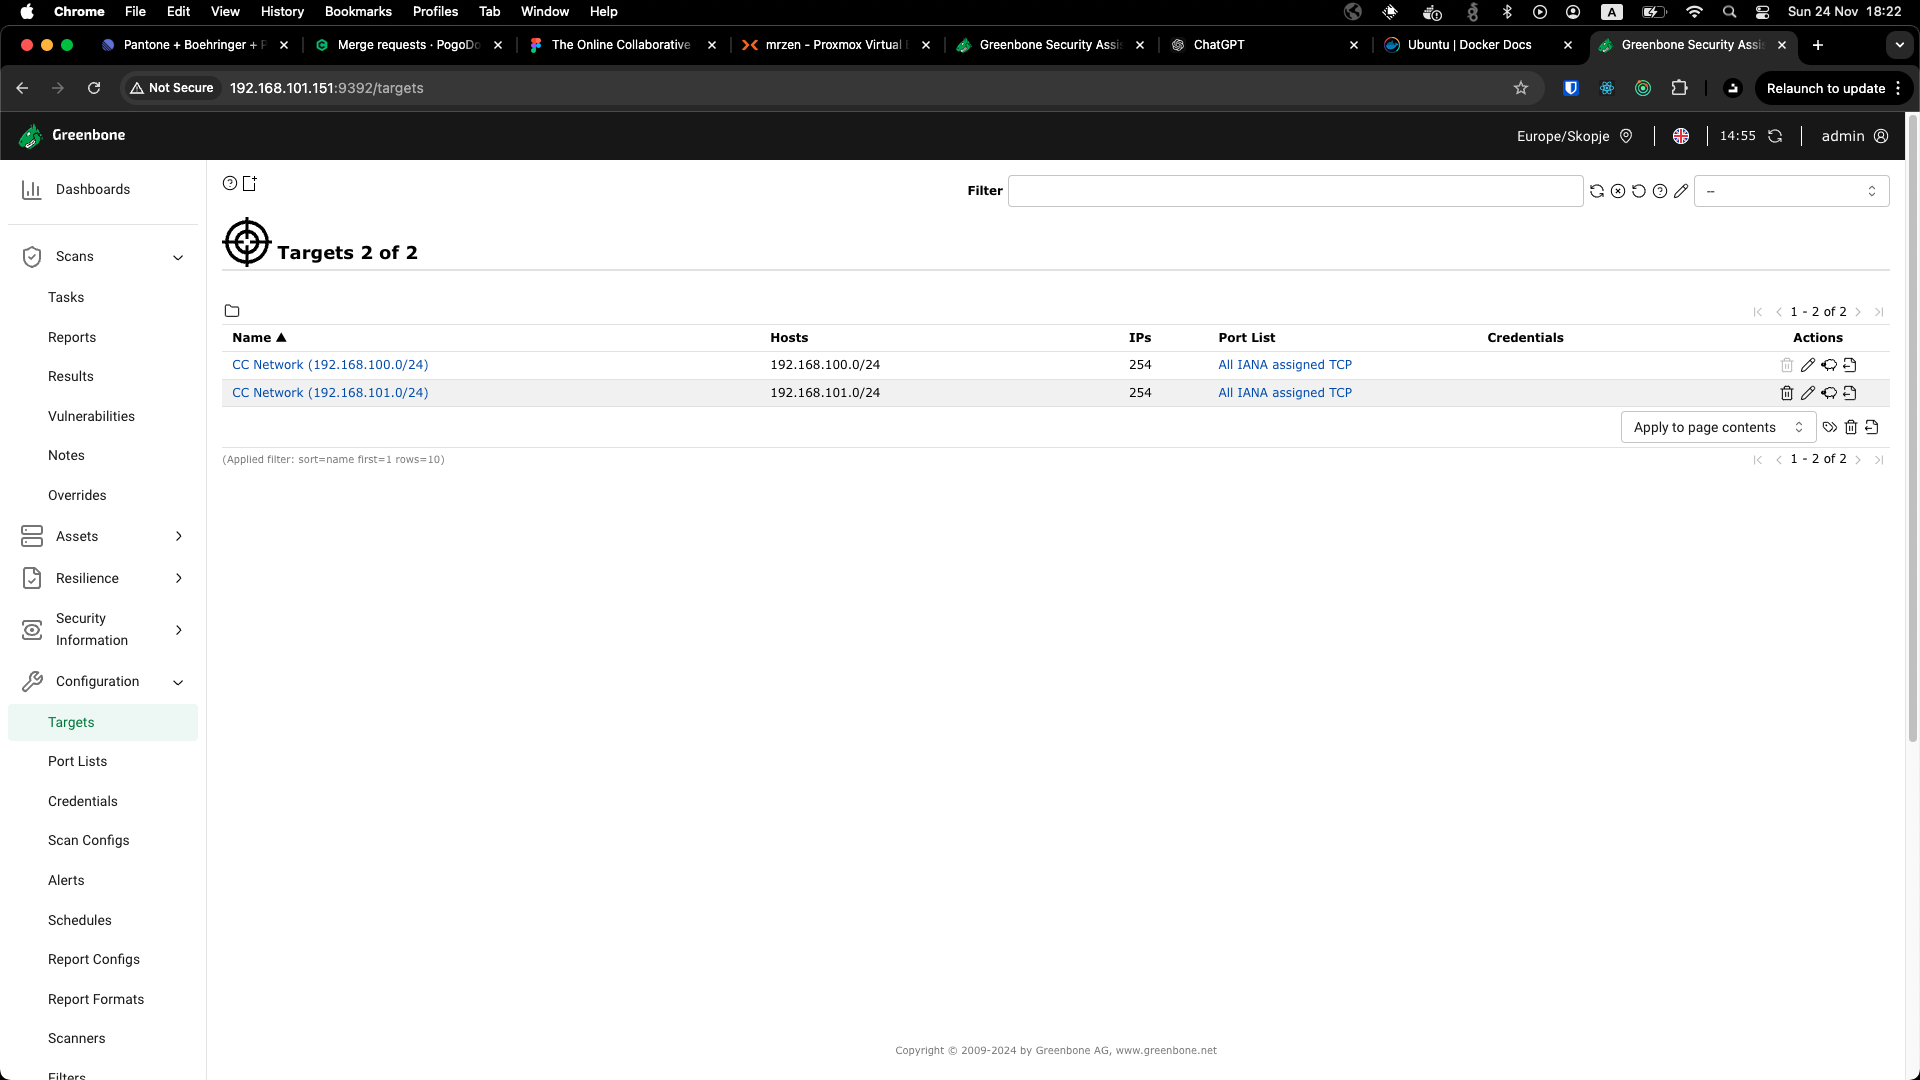
\includegraphics[width=0.5\textwidth]{targets.png}
    \caption{Targets}
\end{figure}

\subsubsection{Host Discovery Task}

With the targets defined, I created the first scan task, which was a \textit{Host Discovery} task (Fig. 7). This task was designed to identify all active hosts within the defined subnets, helping to ensure that no device was overlooked. The host discovery scan was configured without any scheduling or alerts at this stage, as its purpose was solely to gather information about the devices on the network.

\begin{figure}[h!]
    \centering
    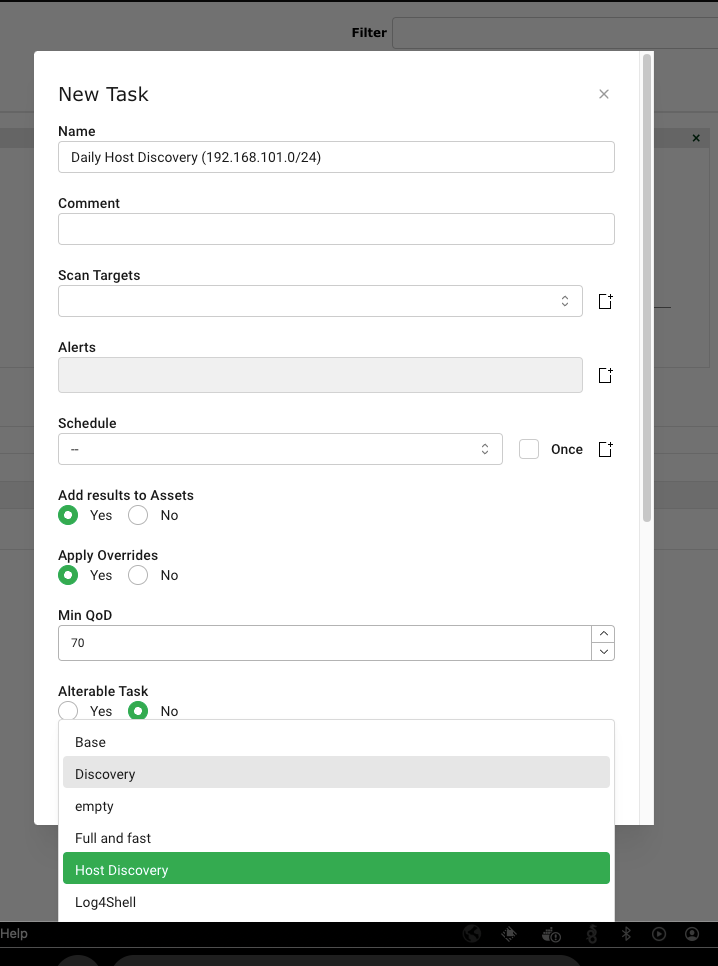
\includegraphics[width=0.5\textwidth]{hosts.png}
    \caption{Host Discovery}
\end{figure}


The scan was initiated for both subnets \texttt{192.168.0.100/24} and \texttt{192.168.0.101/24}. The results of this task showed all of the devices that were actively connected to the network, including servers, workstations, networked devices, and other endpoints. The host discovery task was essential for building a clear inventory of the devices on the network, which would later help identify specific systems to target in the vulnerability scans.

\subsubsection{Full and Fast Scans}

After successfully completing the host discovery task, I proceeded to create the next two scan tasks: \textit{Full and Fast Scan} (Fig. 8). This scan was selected to ensure comprehensive coverage of the devices within the defined subnets and to test for vulnerabilities in the systems.

\textit{Full Scans} were configured to perform a thorough vulnerability assessment, testing every device on the network for security weaknesses. This included scanning for missing patches, configuration errors, open ports, and any other potential vulnerabilities. They were also run to provide a high-level overview of the security posture of the devices. They provided valuable insights into any obvious security risks that needed immediate attention.

\begin{figure}[h!]
    \centering
    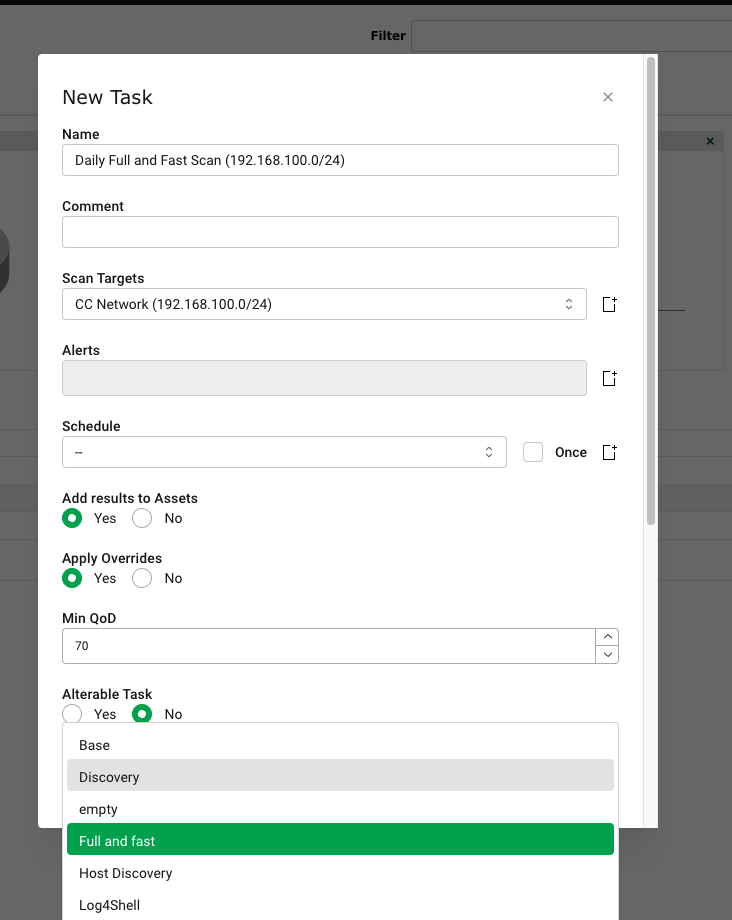
\includegraphics[width=0.5\textwidth]{full.png}
    \caption{Full and Fast Scan}
\end{figure}

The scan was executed across all devices identified during the host discovery phase, and the process took approximately 3-4 hours for one of the subnets. Once the scan was completed, OpenVAS generated detailed reports that outlined the vulnerabilities found on each device. The reports included information about each device's operating system, open ports, installed applications, certificates, and CVEs (Common Vulnerabilities and Exposures). The vulnerabilities were ranked by severity using the CVSS (Common Vulnerability Scoring System), which allowed me to prioritize remediation efforts based on the potential risk posed by each vulnerability.

After the scans were completed, OpenVAS generated a comprehensive vulnerability report that included detailed information about the devices and services within the network (Fig. 9). The report was categorized based on the severity of the vulnerabilities detected, with each finding offering actionable insights for improving the security posture of the network. 

\begin{figure}[h!]
    \centering
    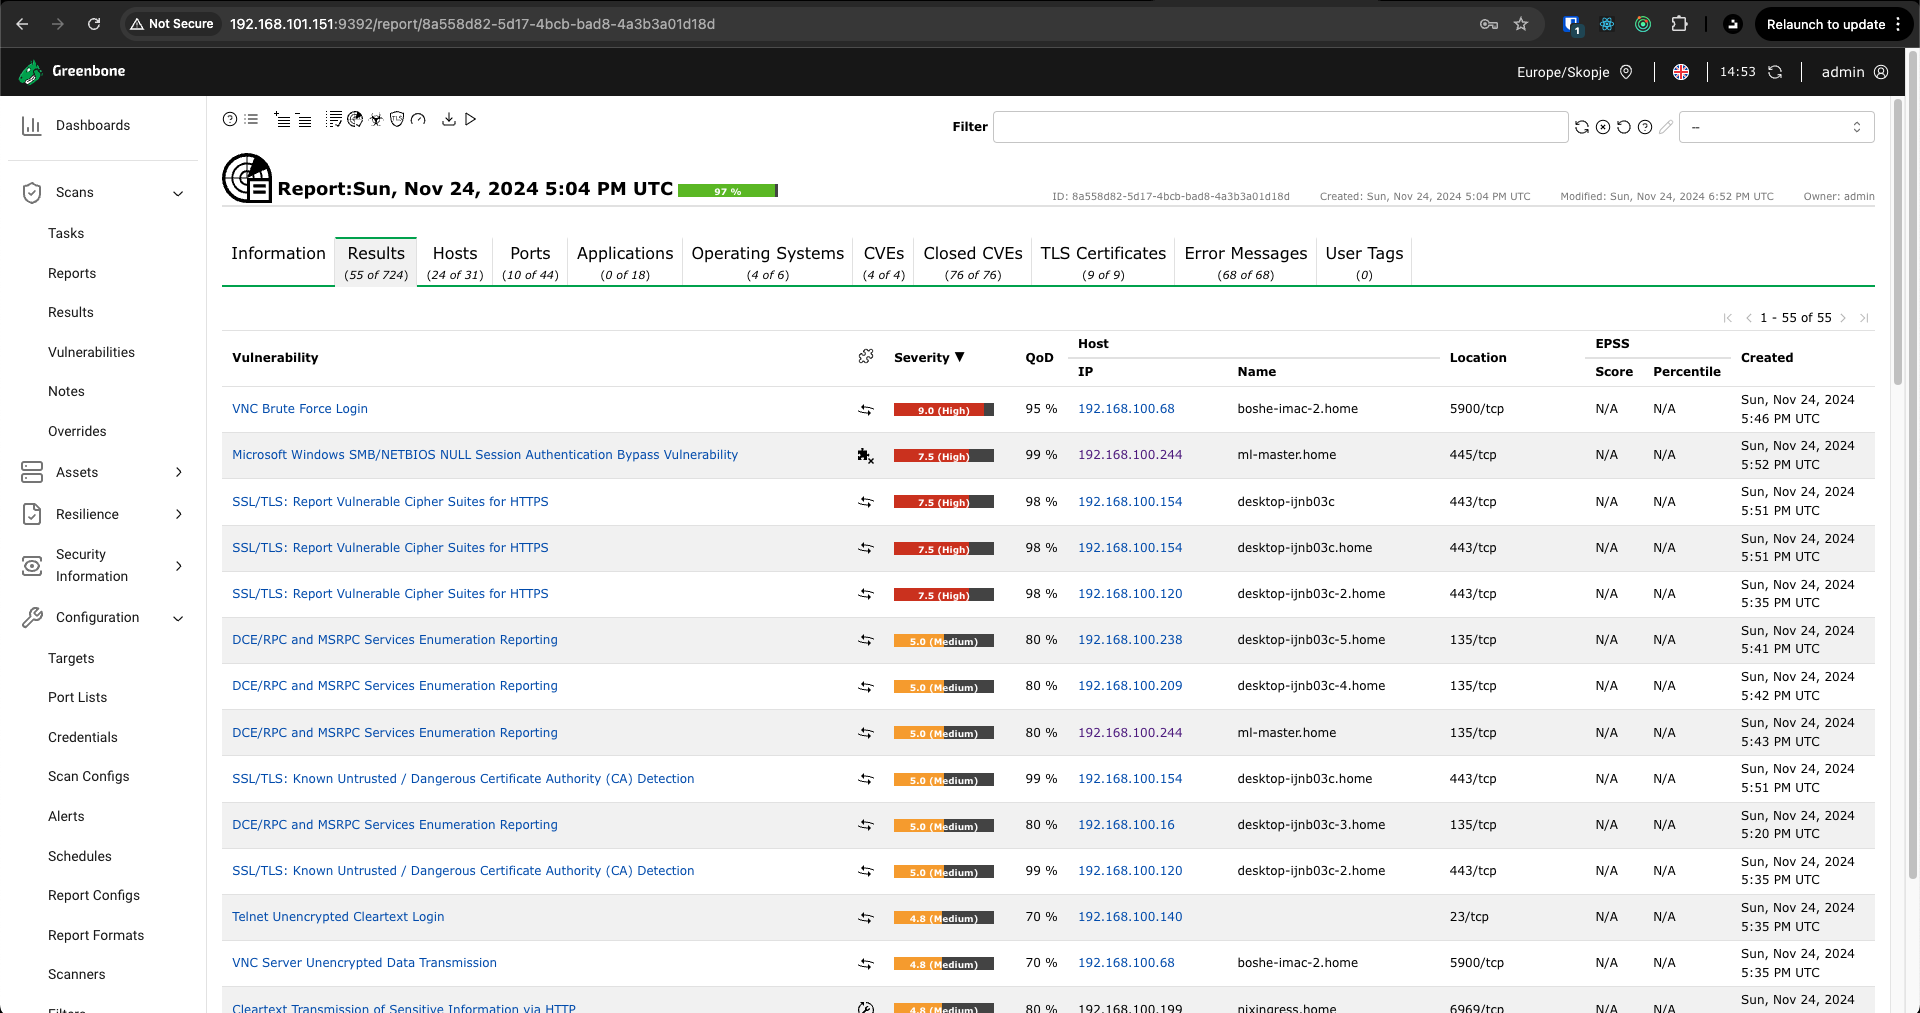
\includegraphics[width=0.5\textwidth]{results.png}
    \caption{Targets}
\end{figure}


One of the key highlights of the report was the detection of a potential brute force login attempt on a device running the VNC Remote Control service. OpenVAS was able to successfully brute-force the VNC password and provide the exact password it used to gain access to the device. This example clearly demonstrates the value of OpenVAS in identifying weak credentials and other vulnerabilities that may go unnoticed without proper scanning.

This was a critical finding, as it highlighted a serious security risk that could have been exploited by an attacker. Had the device remained unmonitored, it is highly likely that an attacker could have gained unauthorized access to sensitive systems. OpenVAS, by identifying this vulnerability and providing the password used in the brute-force attack, allowed us to take immediate action. I was able to use the discovered password to log into the device, demonstrating the severity of the issue. The detailed report not only provided the password itself but also contextualized the risk by explaining how easily an attacker could exploit this vulnerability. By using OpenVAS, we were able to uncover this weak point in our network and quickly address the issue by changing the password to a more secure one. This was a prime example of how OpenVAS can help organizations identify and remediate vulnerabilities that may otherwise remain hidden.

The report also provided information on other vulnerabilities across the network, ranking them based on severity and impact. These results enabled the security team to prioritize the remediation efforts and focus on addressing the most critical vulnerabilities first, which helped strengthen the overall security of the network.

Regarding the Full Scan, OpenVAS provided a thorough and detailed report for each vulnerability that included:

\begin{itemize}
    \item The exact vulnerability
    \item The affected service/host and port
    \item The vulnerability's severity, classified by OpenVAS based on the CVSS (Common Vulnerability Scoring System).
    \item Recommended actions to mitigate the vulnerability
\end{itemize}

\subsubsection{Authenticated Scans}

After the successful completion of the full and fast scans, I moved on to create \textit{Authenticated Scans} for critical systems, such as web servers and databases. These scans required valid credentials to be configured, allowing OpenVAS to perform more in-depth testing on systems by authenticating with the devices and accessing resources that were not available in unauthenticated scans.

Authenticated scans are important because they can identify vulnerabilities that are not visible from the outside (e.g., issues within the system's configuration or security settings that require system-level access). By enabling authenticated scanning, I was able to gain deeper insights into the security of key systems and ensure that potential vulnerabilities, such as misconfigurations or outdated software, were detected.

\subsubsection{CVE Scan Tasks}

In addition to the full and authenticated scans, I created \textit{CVE Scan Tasks} to specifically target known vulnerabilities identified by their CVE identifiers. CVEs are cataloged security vulnerabilities that are widely recognized across the cybersecurity community. These scan tasks focused on verifying that all systems within the network were checked for the latest critical CVEs, ensuring that no known vulnerabilities were present.

The CVE Scan Tasks were particularly important for systems that were exposed to the internet, such as web servers or other publicly-facing services. By specifically targeting CVEs, I ensured that our systems were up-to-date with the latest security patches and that no critical vulnerabilities were left unaddressed.

\subsubsection{Fine-Tuning the Scan Process}

Once the initial scan results were obtained, I fine-tuned the scanning process further to enhance its efficiency and ensure comprehensive coverage. This included adding more custom configurations to address specific needs within our network (Fig. 10).

One of the primary adjustments made was to create a daily scan schedule. I configured OpenVAS to run the scans at 7:00 AM every day, ensuring that the network's devices were continuously monitored for vulnerabilities. This scheduling feature was crucial for automating the scanning process and ensuring that security assessments were regularly performed without manual intervention.

To stay informed about any vulnerabilities detected during the scans, I configured an alert system that would send an email notification whenever vulnerabilities were found. This alert system ensured that I would be promptly notified about critical issues, enabling me to take immediate action and begin the remediation process.

The alert system was designed to send notifications for any vulnerabilities with a severity higher than a certain threshold, ensuring that only critical issues would trigger alerts. This helped minimize unnecessary emails while still ensuring that the most important findings were brought to my attention.

\begin{figure}[h!]
    \centering
    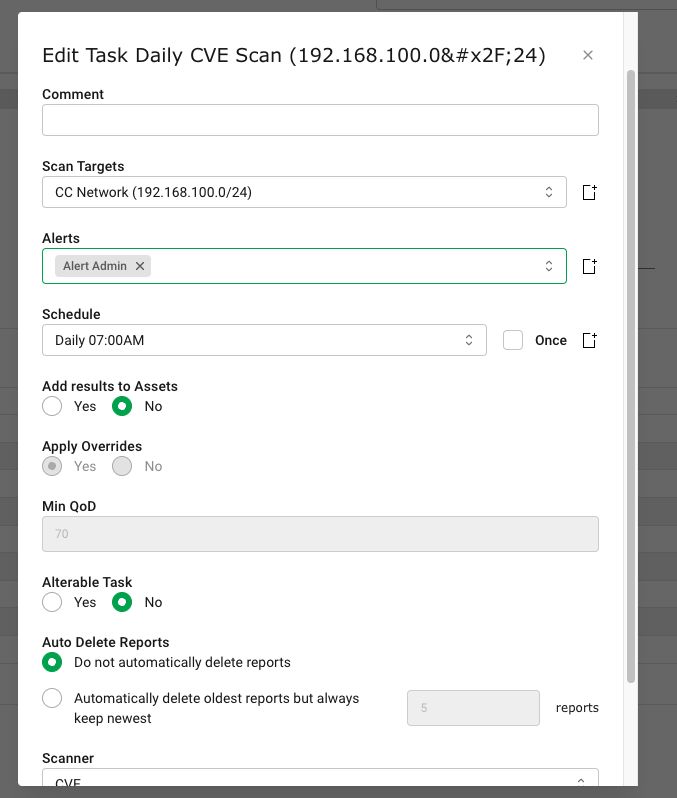
\includegraphics[width=0.5\textwidth]{finetune.png}
    \caption{Alerts and Schedules}
\end{figure}

\subsubsection{Generated Reports and Analysis}

After the completion of each scan, OpenVAS generated extensive reports in PDF format (Fig. 11), which detailed the vulnerabilities found across the network. These reports were comprehensive, listing each identified vulnerability, categorizing it by severity, and providing actionable recommendations for remediation.

The reports included details such as:

\begin{itemize}
    \item A list of all detected vulnerabilities, categorized by severity (Critical, High, Medium, Low)
    \item Recommendations for fixing each vulnerability (e.g., patching software, adjusting configurations)
    \item Risk assessments based on the potential impact of each vulnerability
    \item A summary of the affected systems and applications
\end{itemize}

\begin{figure}[!htbp]
    \centering
    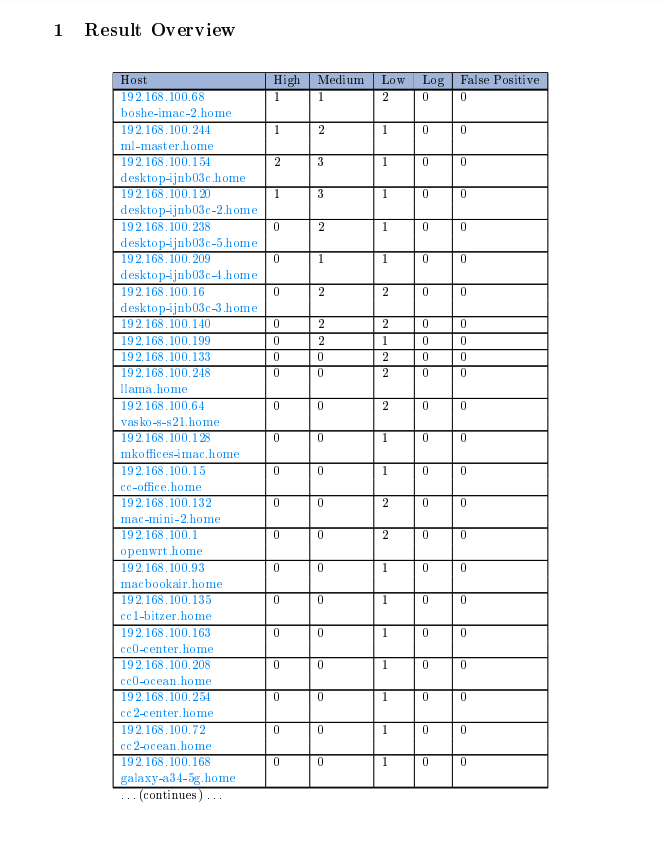
\includegraphics[width=0.5\textwidth]{pdf.png}
    \caption{Result Overview PDF}
\end{figure}

The generated PDF reports were detailed and comprehensive (Fig. 12), containing a wealth of information that could be used by the security team to address vulnerabilities in a systematic and prioritized manner.

\begin{figure}[!htbp]
    \centering
    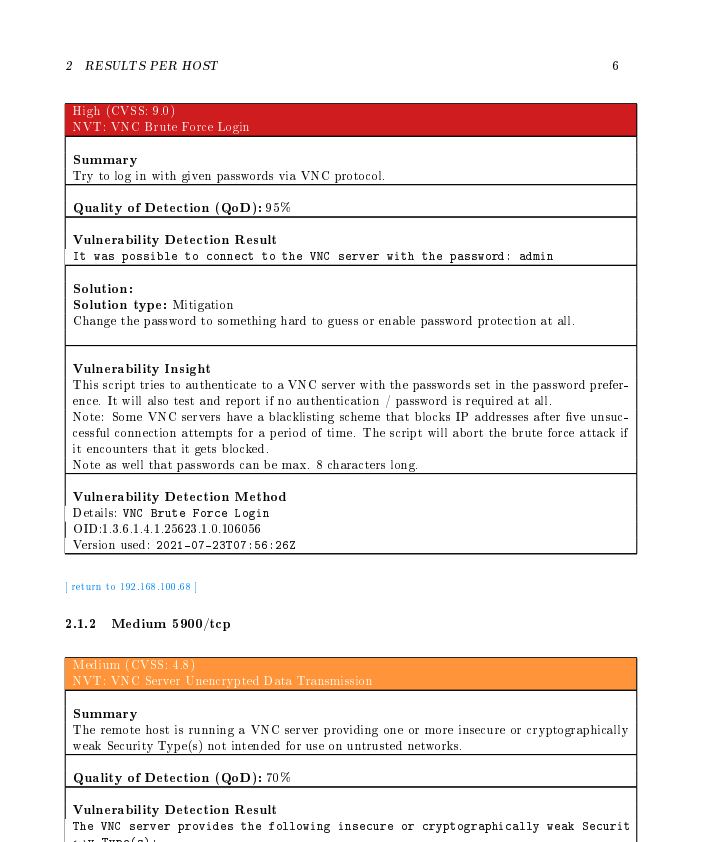
\includegraphics[width=0.5\textwidth]{report.png}
    \caption{Example Result PDF}
\end{figure}

\subsection{Transition to On-Premise Setup}

After successfully testing the scans and fine-tuning the configuration, the next step is to transition the entire OpenVAS setup from a virtual machine (VM) to a dedicated on-premise server. This transition is necessary to ensure that the scans can run reliably on a machine that is always available, without the potential resource limitations or instability of a VM.

Moving OpenVAS to an on-premise machine will enable it to perform daily scans without interruption, providing continuous monitoring of the network's security posture. The on-premise setup will also allow for more control over the hardware resources and ensure that OpenVAS can handle larger networks and scan tasks without performance degradation.

Once the OpenVAS setup was moved to an on-premise server, OpenVAS was successfully setup. In the future, I plan to configure additional automation and reporting features to further streamline the vulnerability management process. These include creating automated remediation workflows and integrating OpenVAS with other security tools within the company's infrastructure to enhance the overall security management system.

The final configuration and setup on the on-premise server were initiated successfully the next day according to the scheduled task (Fig. 13).

\begin{figure}[h!]
    \centering
    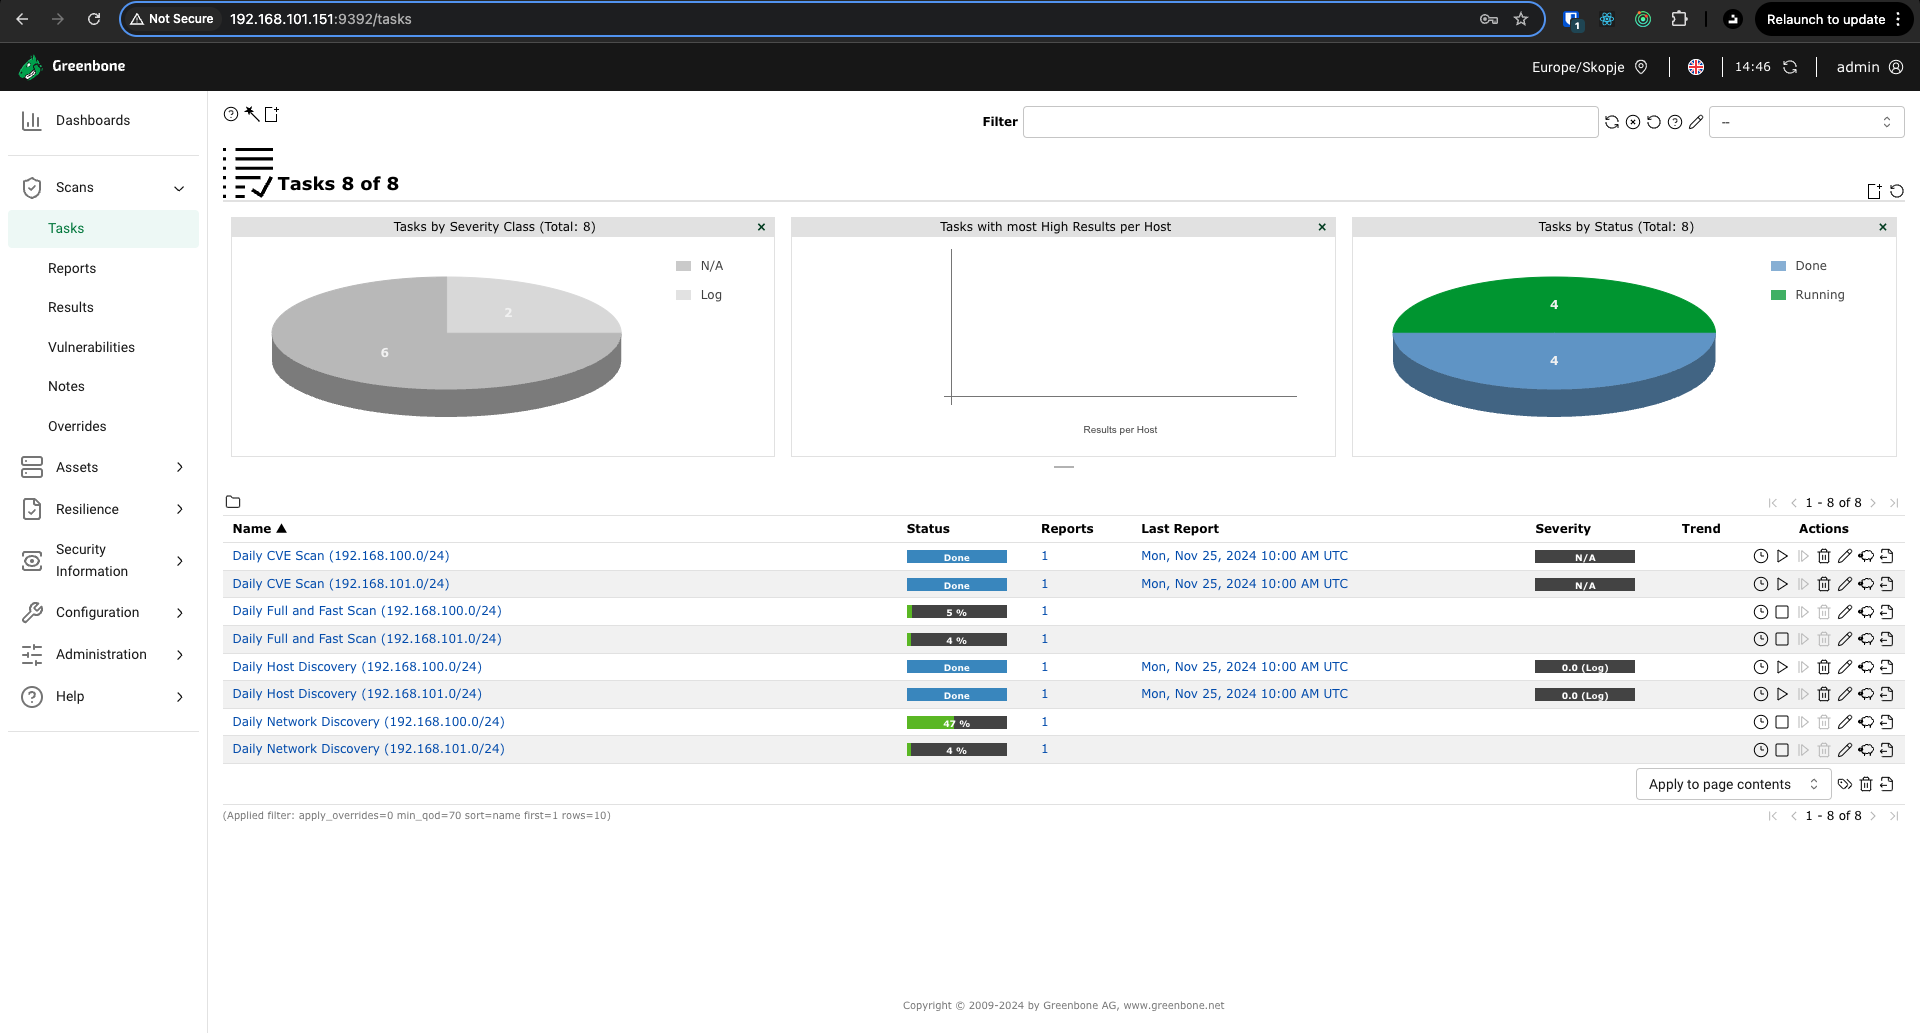
\includegraphics[width=0.5\textwidth]{config.png}
    \caption{Final Configuration}
\end{figure}

\section{Conclusion}

In this paper, I have explored the practical implementation of OpenVAS as a vulnerability scanning and risk mitigation tool within a corporate network environment. Through a detailed deployment process, starting from an initial setup on a macOS machine and eventually transitioning to a dedicated on-premise server, I have demonstrated how OpenVAS can be leveraged to enhance network security. The findings from the vulnerability scans highlighted both critical and minor weaknesses in the network, emphasizing the importance of continuous monitoring and timely remediation of vulnerabilities.

OpenVAS proved to be a powerful tool in identifying security risks, generating actionable insights, and providing recommendations for mitigating those risks. Its ability to conduct full, authenticated, and customized scans allowed for thorough assessments of the network, covering a broad range of vulnerabilities. The detailed reports generated by OpenVAS were invaluable in prioritizing remediation efforts, offering a structured approach to addressing vulnerabilities based on their severity and potential impact on the organization.

While OpenVAS offers significant benefits, including being a cost-effective, open-source solution, it also presents certain challenges. These include performance limitations when scanning large networks, and the need for manual intervention to verify and mitigate false positives. Nonetheless, the flexibility and scalability of OpenVAS make it a crucial component in any organization’s cybersecurity framework, especially when integrated into an automated vulnerability management system.

The transition to an on-premise setup will ensure the reliability and continuity of vulnerability scanning, enabling the organization to maintain a proactive security posture. As OpenVAS becomes an integral part of our ongoing security strategy, the next steps include further automation, deeper integration with other security tools, and continuous tuning of the scanning configurations to adapt to evolving threats. By adopting OpenVAS as part of a comprehensive cybersecurity strategy, organizations can significantly improve their defenses, mitigate risks, and reduce the potential impact of cyber threats.

In conclusion, OpenVAS serves as a valuable resource in securing networks, offering robust vulnerability scanning capabilities, detailed reports, and a user-friendly interface, making it an essential tool for enhancing network security and mitigating potential risks.

\begin{center} \textbf{ACKNOWLEDGEMENT} \end{center}
I would like to express my sincere gratitude to my company CodeChem, for providing me with the opportunity and resources to implement OpenVAS within our network. I am thankful for the trust placed in me to enhancing our network security.

\begin{thebibliography}{99}

\bibitem{openvas}
Greenbone Networks. (2024). \textit{OpenVAS: Open Vulnerability Assessment System}.

\bibitem{cve}
Common Vulnerabilities and Exposures (CVE). (2024). \textit{What is CVE?}.

\bibitem{gvm}
Greenbone Networks. (2024). \textit{Greenbone Vulnerability Management (GVM)}.

\bibitem{aksu2017}
M. U. Aksu, M. H. Dilek, E. I. Tatli, K. Bicakci, H. I. Dirik, M. U. Demirezen, and T. Aykir, “A Quantitative CVSS-Based Cyber Security Risk Assessment Methodology For IT Systems,” in \textit{The 51st International Carnahan Conference on Security Technology}, 2017.

\bibitem{bingham2014}
M. Bingham, A. Skillen, and A. Somayaji, “Even Hackers Deserve Usability: An Expert Evaluation of Penetration Testing Tools,” in \textit{9th Annual Symposium on Information Assurance (ASIA14)}, pp. 13–21, 2014.

\bibitem{yoshimoto2007}
M. Yoshimoto, T. Katoh, B. B. Bista, and T. Takata, “Development and evaluation of new user interface for security scanner with usability in human interface study,” in \textit{1st International Conference on Network-Based Information Systems}, NBiS 2007, vol. 4658 LNCS, pp. 127–136, 2007.

\bibitem{sears1997}
A. Sears, “Heuristic Walkthroughs: Finding the Problems Without the Noise,” \textit{International Journal of Human-Computer Interaction}, 1997.

\bibitem{wang2017}
Y. Wang and J. Yang, “Ethical hacking and network defense: Choose your best network vulnerability scanning tool,” in \textit{Proceedings - 31st IEEE International Conference on Advanced Information Networking and Applications Workshops, WAINA 2017}, pp. 110–113, 2017.

\bibitem{johansson2007}
A. Jøsang, B. AlFayyadh, T. Grandison, M. AlZomai, and J. McNamara, “Security usability principles for vulnerability analysis and risk assessment,” in \textit{Proceedings - Annual Computer Security Applications Conference, ACSAC}, pp. 269–278, 2007.

\bibitem{whitten1999}
A. Whitten and J. Tyger, “Why Johnny Can’t Encrypt: A Usability Evaluation of PGP 5.0,” in \textit{the 8th USENIX Security Symposium}, 1999.

\bibitem{mack1992}
R. L. Mack and J. Nielsen, “Usability Inspection Methods,” in \textit{SIGCHI ’92}, vol. 25, no. 1, pp. 28–33, 1992.

\bibitem{schmettow2012}
M. Schmettow, “Sample size in usability studies,” \textit{Communications of the ACM}, vol. 55, no. 4, p. 64, 2012.


\end{thebibliography}

\end{document}

